\chapter{Хильбудийщина}

Раньше дети играли в «испорченный телефон». Один говорит на ухо слово другому, тот, что ему послышалось – соседу, а сосед – своему соседу. И последний в цепочке сообщает, что же получилось. А за ним и первый объявляет. Бывает смешно.

С полной серьезностью в испорченный телефон играют историки. Игра продолжается, снежный ком небылиц увеличивается, катится, по нему, как по глобусу, пишут научные труды.

На арену вопроса основания Киева ученые вывели Хильбудия, чье имя мелькнуло в истории касательно войны Византии с Готами. Полагают, будто Хильбудий – это Кий, либо его прообраз. Хильбудий стал героем современных романов на исторические темы, проник в статьи да учебники. Повсюду и без вопросов. Пора их задать.

Кто такой Хильбудий?

Прокопий Кесарийский (Procopius Caesariensis, 500\ – 565) в «Готской войне»\cite{procopius01}  мимоходом сообщает о византийском военачальнике по имени Хилвоудиос (Χιλβου\-διος, Хильбудий в общепринятом переложении), жившем в 6-м веке, при императоре Юстиниане. Познакомимся с этими сведениями в русском переводе\cite{procopius02}. Я не счел отрывок достаточно важным, чтобы переводить его самому, хотя подлинник отличен не только именованиями, которые оказались искажены, а именно, в греческом тексте вместо Славян – Склавы, Хильбудий – Хилвоудиос, Гунны – Оунны, Римляне – Романы.

Прочтем, что же сказано о Хильбудии.

\begin{quotation}
Перезимовав там, с наступлением весны они (герулы и Нарзес) собирались отправиться к Велизарию. С ними был и Иоанн, которому дано было прозвище Фага\footnote{Обжора.}. На этом пути им было суждено совершенно неожиданно оказать римлянам великое благодеяние.

Случилось, что незадолго перед тем большой отряд славян, перейдя реку Истр, стал грабить тамошние места и забрал в рабство большое количество римлян. Герулы неожиданно напали на них и сверх ожидания победили их, хотя славяне намного превосходили их численностью. Они перебили их, а всех пленных римлян отпустили, чтобы они возвратились домой.

Захватив тут некоего человека, присвоившего себе имя Хильбудия, человека знатного, некогда бывшего у римлян претором – начальником войска, Нарзес легко уличил его в самозванстве. Как это все было, я сейчас расскажу.

Был некто Хильбудий, близкий к императорскому дому, в военном деле человек исключительно энергичный, и настолько выше жажды стяжательства, что вместо величайших богатств он по существу не приобрел никакого состояния. На четвертом году своей единодержавной власти император, назначив этого Хильбудия начальником Фракии, поставил на охрану реки Истра, приказав ему стеречь, чтобы жившие там варвары не могли уже переходить реку. 

Дело в том, что жившие по Истру варвары, гунны, анты и славяне, часто совершая такие переходы, наносили римлянам неисцелимый вред. Хильбудий настолько был страшен варварам, что в течение трех лет, пока он там был, облеченный званием военачальника, не только никто из варваров не осмеливался перейти Истр для войны с римлянами, но сами римляне под начальством Хильбудия, неоднократно переходя в земли по ту сторону реки, избивали и забирали в рабство живших там варваров.

Спустя три года после своего прибытия Хильбудий по обычаю перешел реку с небольшим отрядом, славяне же выступили против него все поголовно. Битва была жестокая: пало много римлян, в том числе и их начальник Хильбудий. 

В дальнейшем река навсегда стала доступной для переходов варваров по их желанию и римская область совершенно открыта для их вторжений. Таким образом, все могущество Римской империи в этом деле оказалось совершенно неравносильным доблести одного человека.

Спустя некоторое время анты и славяне рас\-сорились между собой и вступили в войну. Случилось так, что в этой войне анты были побеждены врагами. В этом столкновении один славянин взял в плен из числа врагов юношу, едва достигшего зрелости, по имени Хильбудий, и отвел его к себе домой. С течением времени этот Хильбудий оказался очень расположенным к своему хозяину и в военном деле очень энергичным. Не раз подвергаясь опасностям за своего господина, он совершил много славных подвигов и смог добиться для себя великой славы.

Около этого времени анты сделали набег на Фракийскую область, и многих из бывших там римлян ограбили и обратили в рабство. Гоня их перед собою, они вернулись с ними на родину. Одного из этих пленников судьба привела к человеколюбивому и мягкому хозяину. Сам же этот человек был очень коварен и способен обмануть любого встречного. Так как при всем желании он не находил никаких средств вернуться в римскую землю, он придумал следующее. 

Придя к хозяину, он рассыпался в похвалах его милосердию и утверждал, что за это ему от бога будет много всяких благ, что сам он ни в коем случае не окажется неблагодарный своему добрейшему господину и что если тот захочет послушать его добрых советов, которые он очень хорошо придумал, то в скором времени он сделает его обладателем большой суммы денег. 

На его вопросы, как это будет, он сказал, что у одного из славянских племен на положении раба находится Хильбудий, бывший военачальником римлян, скрывающий от всех варваров, кто он такой. Если таким образом ему будет угодно выкупить Хильбудия и доставить его в землю римлян, то вполне естественно, что он получит великую славу и очень много денег от императора. Такими речами римлянин тотчас убедил своего хозяина и вместе с ним отправился к славянам.

У этих народов был заключен мирный договор, и они без страха общались друг с другом. И вот, предложив хозяину Хильбудия большую сумму, они купили этого человека и с ним быстро вернулись домой. Когда они вернулись к себе, в свое местожительство, купивший стал его спрашивать, правда ли, что он Хильбудий, римский военачальник. 

Он не отказался рассказать все, как было, и со всей откровенностью изложил по порядку всю свою жизнь, что и он сам по роду ант, что, сражаясь вместе со своими родичами против славян, бывших тогда их врагами, был кем-то из неприятелей взят в плен, теперь же, придя в родные земли, он в дальнейшем, согласно закону, будет уже свободным.

Заплативший за него деньги остолбенел, лишившись речи от изумления, и впал в величайший гнев, лишившись столь великой надежды на выгоду. Но римлянин, желая его утешить и скрыть истину, чтобы не сделать своего возвращения домой более затруднительным, продолжал настаивать, что этот человек – тот самый (римский) Хильбудий, но что он, находясь в среде варваров, боится и потому меньше всего желает открыть все, когда же он окажется в римской земле, то не только не будет скрывать правды, но, естественно, будет еще гордиться этим именем. И вначале все это делалось тайно от остальных варваров.

Когда этот слух, распространяясь в народе, стал достоянием всех, то по этому поводу собрались почти все анты, считая это дело общим и полагая, что для них всех будет большим благом то, что они – хозяева римского полководца Хильбудия.
\end{quotation}

А также:

\begin{quotation}
Собравшись, как сказано выше, анты заставили этого человека признать, как они хотели, что он – Хильбудий, римский военачальник. Они грозили, что накажут его, если он будет это отрицать.

Как раз тогда, когда все это происходило, в это время император Юстиниан, отправив некоторых лиц послами к этим варварам, предлагал им поселиться в древнем городе, по имени Туррис, расположенном (севернее) за рекой Истром. В прежние времена этот город построил римский император Траян, но уже издавна этот город был покинутым, так как местные варвары его всегда разграбляли. Император Юстиниан соглашался одарить их этим городом и окружающей его областью, так как искони она принадлежала римлянам, обещал, что будет жить с ними, всячески стараясь сохранить мир, и даст им много денег с тем только, чтобы на будущее время они клятвенно обещали соблюдать с ним мир и всегда препятствовали гуннам, когда они захотят сделать набег на Римскую империю.

Варвары все это выслушали, одобрили и обещали сделать все это, если он восстановит начальником римского вождя Хильбудия и даст ему жить вместе с ними, утверждая, как они и задумали, что этот человек и есть Хильбудий. Возымев надежды на столь высокое положение, уже и сам этот человек пожелал быть им и утверждал, что он – Хильбудий, римский военачальник.

Отправленного с этой целью в Византию Нарзес захватил на этом пути. Встретившись с ним и найдя, что он обманщик (хотя он говорил на латинском языке и искусно притворялся, узнав уже наперед многое из того, чем можно было узнать в нем Хильбудия), он заключил его в тюрьму и принудил рассказать все дело. После этого отступления я возвращаюсь к продолжению своего рассказа.
\end{quotation}

Несколько примечаний. 

Уточню концовку по подлиннику – Нарзес доставляет лже-Хильбудия в цепях в Византию для обличения самозванства. Везде говорится о Римлянах потому, что те, кого ученые именуют Византийцами, называли и считали себя Римлянами, Ромеями, гражданами Римской империи. Ибо это позже ученые искусственно разделили Римскую империю и Византийскую, положив временным разделом перенос императором Константином столицы из Рима в Византий (Константинополь, Стамбул). 

Кстати, Константин переименовал Византий в Новый Рим. До 7 века государственным языком Византии считалась латынь. Латынь была в обиходе при дворе императора, в администрации и армии. Разговорным же языком на землях, близких к новой столице, был преимущественно греческий. Впрочем, всё зависело от местного населения.

Как бы ни было, при Юстиниане латынь использовалась «верхушкой». Судя по сведениям Прокопия, лже-Хильбудий говорил на латыни, тем самым выдавая себя за настоящего претора. Кто тогда использовал латынь, кроме самих, условно говоря, Ромеев? Кое-кто по Дунаю, есть даже термин «балканская латынь». Но уж латынь точно не была родным языком Антов. Прокопий писал, что у Склавов и Антов язык одинаковый.

Итак, два Хильбудия – один римский военачальник, и выдающий себя за него одноименный Ант. Из какого народа был первый, неясно.

Поведанные Прокопием события из жизни этих Хильбудиев показались Борису Рыбакову схожими с короткой историей о хождении Кия к цесарю и посещении Дуная, которую изложил Нестор:

\begin{quotation}
яко велику честь приял есть от цесаря, которого не вем и при котором приходи цесари. Идущю же ему опять, приде к Дунаеви, и возлюби место, и сруби городок мал, и хотяше сести с родом своим, и не даша ему близ живущии.
\end{quotation}

Но что тут общего с рассказом про Хильбудиев? Река Истр – Дунай. На нем, по Нестору, Кий городок срубил, да местные прогнали. Рыбаков из одной научной работы в другую на разные лады говорил о Хильбудии. Выражаемые академиком взгляды менялись. В 1980 году в статье в «Город Кия» он, пересказав Прокопия, делал вывод: 

\begin{quotation}
Летописный рассказ о князе Кие находит почти полную параллель в повествовании византийского историка Прокопия Кессарийского. 
\end{quotation}

Спустя два года, в объемном труде «Киевская Русь», уже помягче: 

\begin{quotation}
Нельзя отождествлять Хильбудия с Кием и Туррис с Киевцем, но, очевидно, что сказание о Полянском (антском) князе Кие хронологически надо сближать с эпохой Юстиниана, когда империя была заинтересована в том, чтобы поселить на дунайской границе те или иные славянские дружины, заключив с ними договор о защите империи от других славян и кочевников, за что и приходилось «давать им много денег», оказывать им «великую честь».
\end{quotation}

Каким образом выведено, будто Поляне это Анты? При помощи скобок. А мне понадобилось несколько здоровенных глав насытить выдержками из давних источников, чтобы иметь основание нащупать родство между Полянами и Антами через Аланов и Вандов. Научный метод много проще! Довольно заключить слово в скобки.

А разве летопись сообщает, что Юстиниан или другой василевс намеревался поселить Кия на Дунае? Нет. Тем более, что из летописи явствует – для дунайцев Кий был чужаком, местные не дали ему там обосноваться. В то время как Юстиниан собирался подарить местному антскому населению крепость, лишь бы те в случае чего пособили против Гуннов.

Ученые с подачи Рыбакова восприняли Хильбудия по-своему. Некоторые усмотрели намек, на знак равенства между Кием и Хильбудием. А довод в пользу этому открылся неожиданно, из старой публикации.

В 1902 году, в LXII томе «Периодическо списание на Българското книжовно дружество в София» болгарский ученый Йордан Иванов (1872-1947) поместил короткую заметку «Надгробният надпись на Хилвуда».

Содержание примерно таково. Во-первых, претор Хилвуд (как в статье) именуется Славянином. Однако у Прокопия, Склавы и Анты всё-таки различаются и даже воюют друг с другом, хотя общаются на одном языке. У Иванова же Хилвуд – выслужился, сражается против соплеменников. Кратко введя читателя в курс дела, сочинитель берет быка за рога.

Стамбульская газета Le Moniteur Oriental сообщила, что в Фенере (район Константинополя) при раскопках основания давнего греческого здания нашли мраморный крест с эпитафией. Дается текст на смеси букв греческого и латинского алфавитов. Так ли написано в Le Moniteur Oriental, либо в подлиннике, я не знаю. Вот что приводит Иванов:

\begin{center}
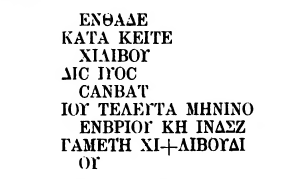
\includegraphics[width=0.50\linewidth]{chast-colebanie-osnov/hilbudiy/hilep.png}
\end{center}

И восстанавливает надпись следующим образом: 
\begin{otherlanguage}{greek}
\begin{quotation}
Ενθαδε χαταχειται Χιλιβουιδισ γιός Σανβατιον τελεν\-τα  μηνι νοέμβριον χη INΔE Z' Γαμετη Χιλιβουι\-διν
\end{quotation}
\end{otherlanguage}

То бишь, в переложении на болгарский:

\begin{quotation}
Тук почива Хиливудъ, синъ Санбатовъ, починал на месеце ноември 28-й, индиктион 7-и. Съпругата на Хиливуда.
\end{quotation}

Что означает:

\begin{quotation}
Тут покоится Хиливуд, сын Санбата, почивший 28 ноября месяца, 7-го индиктиона. Супруга Хиливуда.
\end{quotation}

Что же, исходник предъявлен, другого не будет. Толкование Иванова можно принять или оспорить. Я бы только по сходству имен не решился связать Хильбудия из повествования Прокопия с тем, чью могилу потревожили при раскопках дома.

Но Иванов делает следующие выводы. Упомянутый Прокопием Хилвуд (не уточняется какой, лже или претор) именовался своими домашними Хиливудом. Был погребен в Царьграде. Был сыном Санбатиоса, имя коего по-староболгарски звучало как Собат. Претор Хилвуд служил при императоре Юстиниане, отца коего звали Саббатиос (Sabbatius на латыни). Иванов говорит, что и тот носил славянское имя Собат, переданное византийцами как Саббатиос. Хилвуд был женат, исповедовал христианство, сражение между Славянами и Хилвудом случилось 28 ноября. Год сражения по Прокопию был 534, а по индикту выходит 529.

К слову, позже ученые вычислили год смерти «Хилвуда» иначе. Я уже рассказывал, что такое индикты, и что без дополнительных сведений о событии невозможно установить год по индикту. Это не смутило историков. Они просто решили датировать крест 6-м веком. И стали подсчитывать, когда в том веке был каждый седьмой индикт после смерти настоящего претора Хильбудия (считая 533 за год его гибели).

Седьмые индикты в 6-м веке, по научным таблицам, приходились на 543, 558, 573 и 588 годы. Поэтому ученые говорят, что крест стоял на могиле лже-Хильбудия, либо даже какого-то дополнительного Хильбудия, неведомого науке. 

Что до имени отца покойного, то подобные были тогда в ходу. Не только отец Юстиниана носил это имя. У византийского императора Льва Армянина был сын по имени Symbatios, он же Sabbatios и Sambates – от армянского Smbat. В Армении и цари такие правили – Смбат I, Смбат II.

Но при чем здесь Кий? А вот мол, Константин Багрянородный писал о киевской крепости Самватас. И отчество «Санбат» с надгробия «Хилвуда» – это не имя отца покойного, однако город, откуда Хилвуд родом. Древние иногда употребляли выражение «сын такого-то города или местности» в качестве прозвища. Такой-то сын Афин. Он же такой-то Афинский. А тут родился человек в крепости, всю жизнь нес потом за собой прозвище.

Как мы знаем, претор Хилвоудиос погиб. Вероятно, тело его не нашли, что дало возможность явиться лже-Хильбудию, придунайскому Анту. Разве крепость Самватас стояла на Дунае? Нет. Нет и оснований называть лже-Хильбудия сыном крепости Самватаса. А римского Хильбудия? Это вопрос к ученым, я не знаю, кого они полагают в могиле из статьи Йордана Иванова. Они вроде договорились между собой, что там погребен лже-Хильбудий или совсем другой Хильбудий.

Но чтобы там был похоронен именно Ант Хильбудий, необходимо, дабы по прибытии лже-Хильбудия в Константинополь, мошенника пощадили, а потом он еще и женился – ибо крест поставлен его супругой! Либо вдруг оказалось, что лже-Хильбудий является претором Хильбудием, который чудом выжил, но соблюдал двойную конспирацию. 

Для принятия истинности этого надо сделать слишком много допущений. Я себе не могу такого позволить. Наука – может. Благодаря чему, по меньшей мере само предание о Кие отодвинули во времена Юстиниана, когда, видите ли, Антов хорошо принимали при дворе византийских императоров! Чудодейственная сила скобок, волей которых Кий превратился в Анта, и продолжаем шить суровой ниткой связь времен и событий. Вот в 1980 году отмечали полуторатысячелетний юбилей Киева. Откуда дата? 

Нашли на Замковой горе монеты василевса Анастасия, их датируют шестым веком. Рыбаков связывал наличие этих монет не с торговлей, однако с некими походами Славян на Византию. В статье «Город Кия» академик говорит, как о данности, про заключение союза Кия с византийским императором, легким росчерком пера освобождает историю от братьев Кия и подтягивает датировку: 

\begin{quotation}
В итоге можно сделать следующий вывод: летописный рассказ Нестора о князе Кие (освобожденный от созданной эпическим законом тройственности его братьев) может быть с достаточной убедительностью отнесен не к IX в., как это сделал пристрастный новгородский книжник, а по крайней мере ко времени на три сотни лет раньше – к VI в. нашей эры.
\end{quotation}

О каком новгородском книжнике идет речь? В Новгородской Первой Летописи Младшего Извода основание Киева датировано 854 годом, а научной средой считается, что новгородцы врали, стремясь выставить Новгород древнее Киева. Под давлением этого мнения любые сведения от «новгородцев», не согласующиеся с киевской версией, относят к выдумкам.

«Пристрастный новгородский книжник» сообщил:

\begin{quotation}
В лето 6352 (854). Начало земли Рускои. Живяху кождо с родом своим на своих местех и странах, владеюща кождо родом своим. И быша три братия: единому имя Кии, второму же имя Щек, третьему же имя Хорив, а сестра их Лыбедь. И седяше Кый на горе, идеже ныне увоз Боричев, и бе с родом своим; а брат его Щек на друзии горе, от него же прозвася Щековица; а третии Хорив, от него же прозвася Хоривица. И сотвориша градок, во имя брата своего стареишаго и наркоша имя Кыев.
\end{quotation}

То же, что в других списках, но с привязкой к дате. Ученые ведь придают датам значение, хотя ежели дата не годится, объявляют ложной, не разобравшись.

Но я не буду про числа, это пустое. Вот местность – другое дело, она вещественна, по ней можно пройтись, пощупать землю. Хотя наука умеет сомневаться в несомненном и переиначивать всё в угоду определенным представлениям. Заключать в скобки.

До устроения города Киева, Кий поселился на горе, где при Несторе был увоз Боричев. И хотя поныне в народе бытует представление о Боричеве как о склоне Старокиевского холма, с той стороны, где проложен фуникулер, некоторые ученые пишут такое: «Боричев увоз (современный Андреевский спуск)».
